\documentclass[../main.tex]{subfiles}
 
\begin{document}
 
\begin{figure}[bh]
\centering
 
\end{figure}

\subsection{Definicja problemu}

Podany jest zbiór dróg oraz informacja o tym, które drogi się ze sobą przecinają. Drogi są podzielone na odcinki.
Droga majnastępujące parametry:

\begin{enumerate}  
\item Unikalny numer
\item Rozmiar - liczba odcinków
\item Informacja o tym, z którymi drogami się przecina oraz w którym odcinku
\end{enumerate}


Podany jest zbiór aut, które mają następujące parametry:

\begin{enumerate}  
\item Unikalny numer auta
\item Numer drogi na której się znajduje
\item Numer odcinku drogi na której się znajduje
\item Aktualna prędkość
\end{enumerate}


%Wizualizacja modelu:

%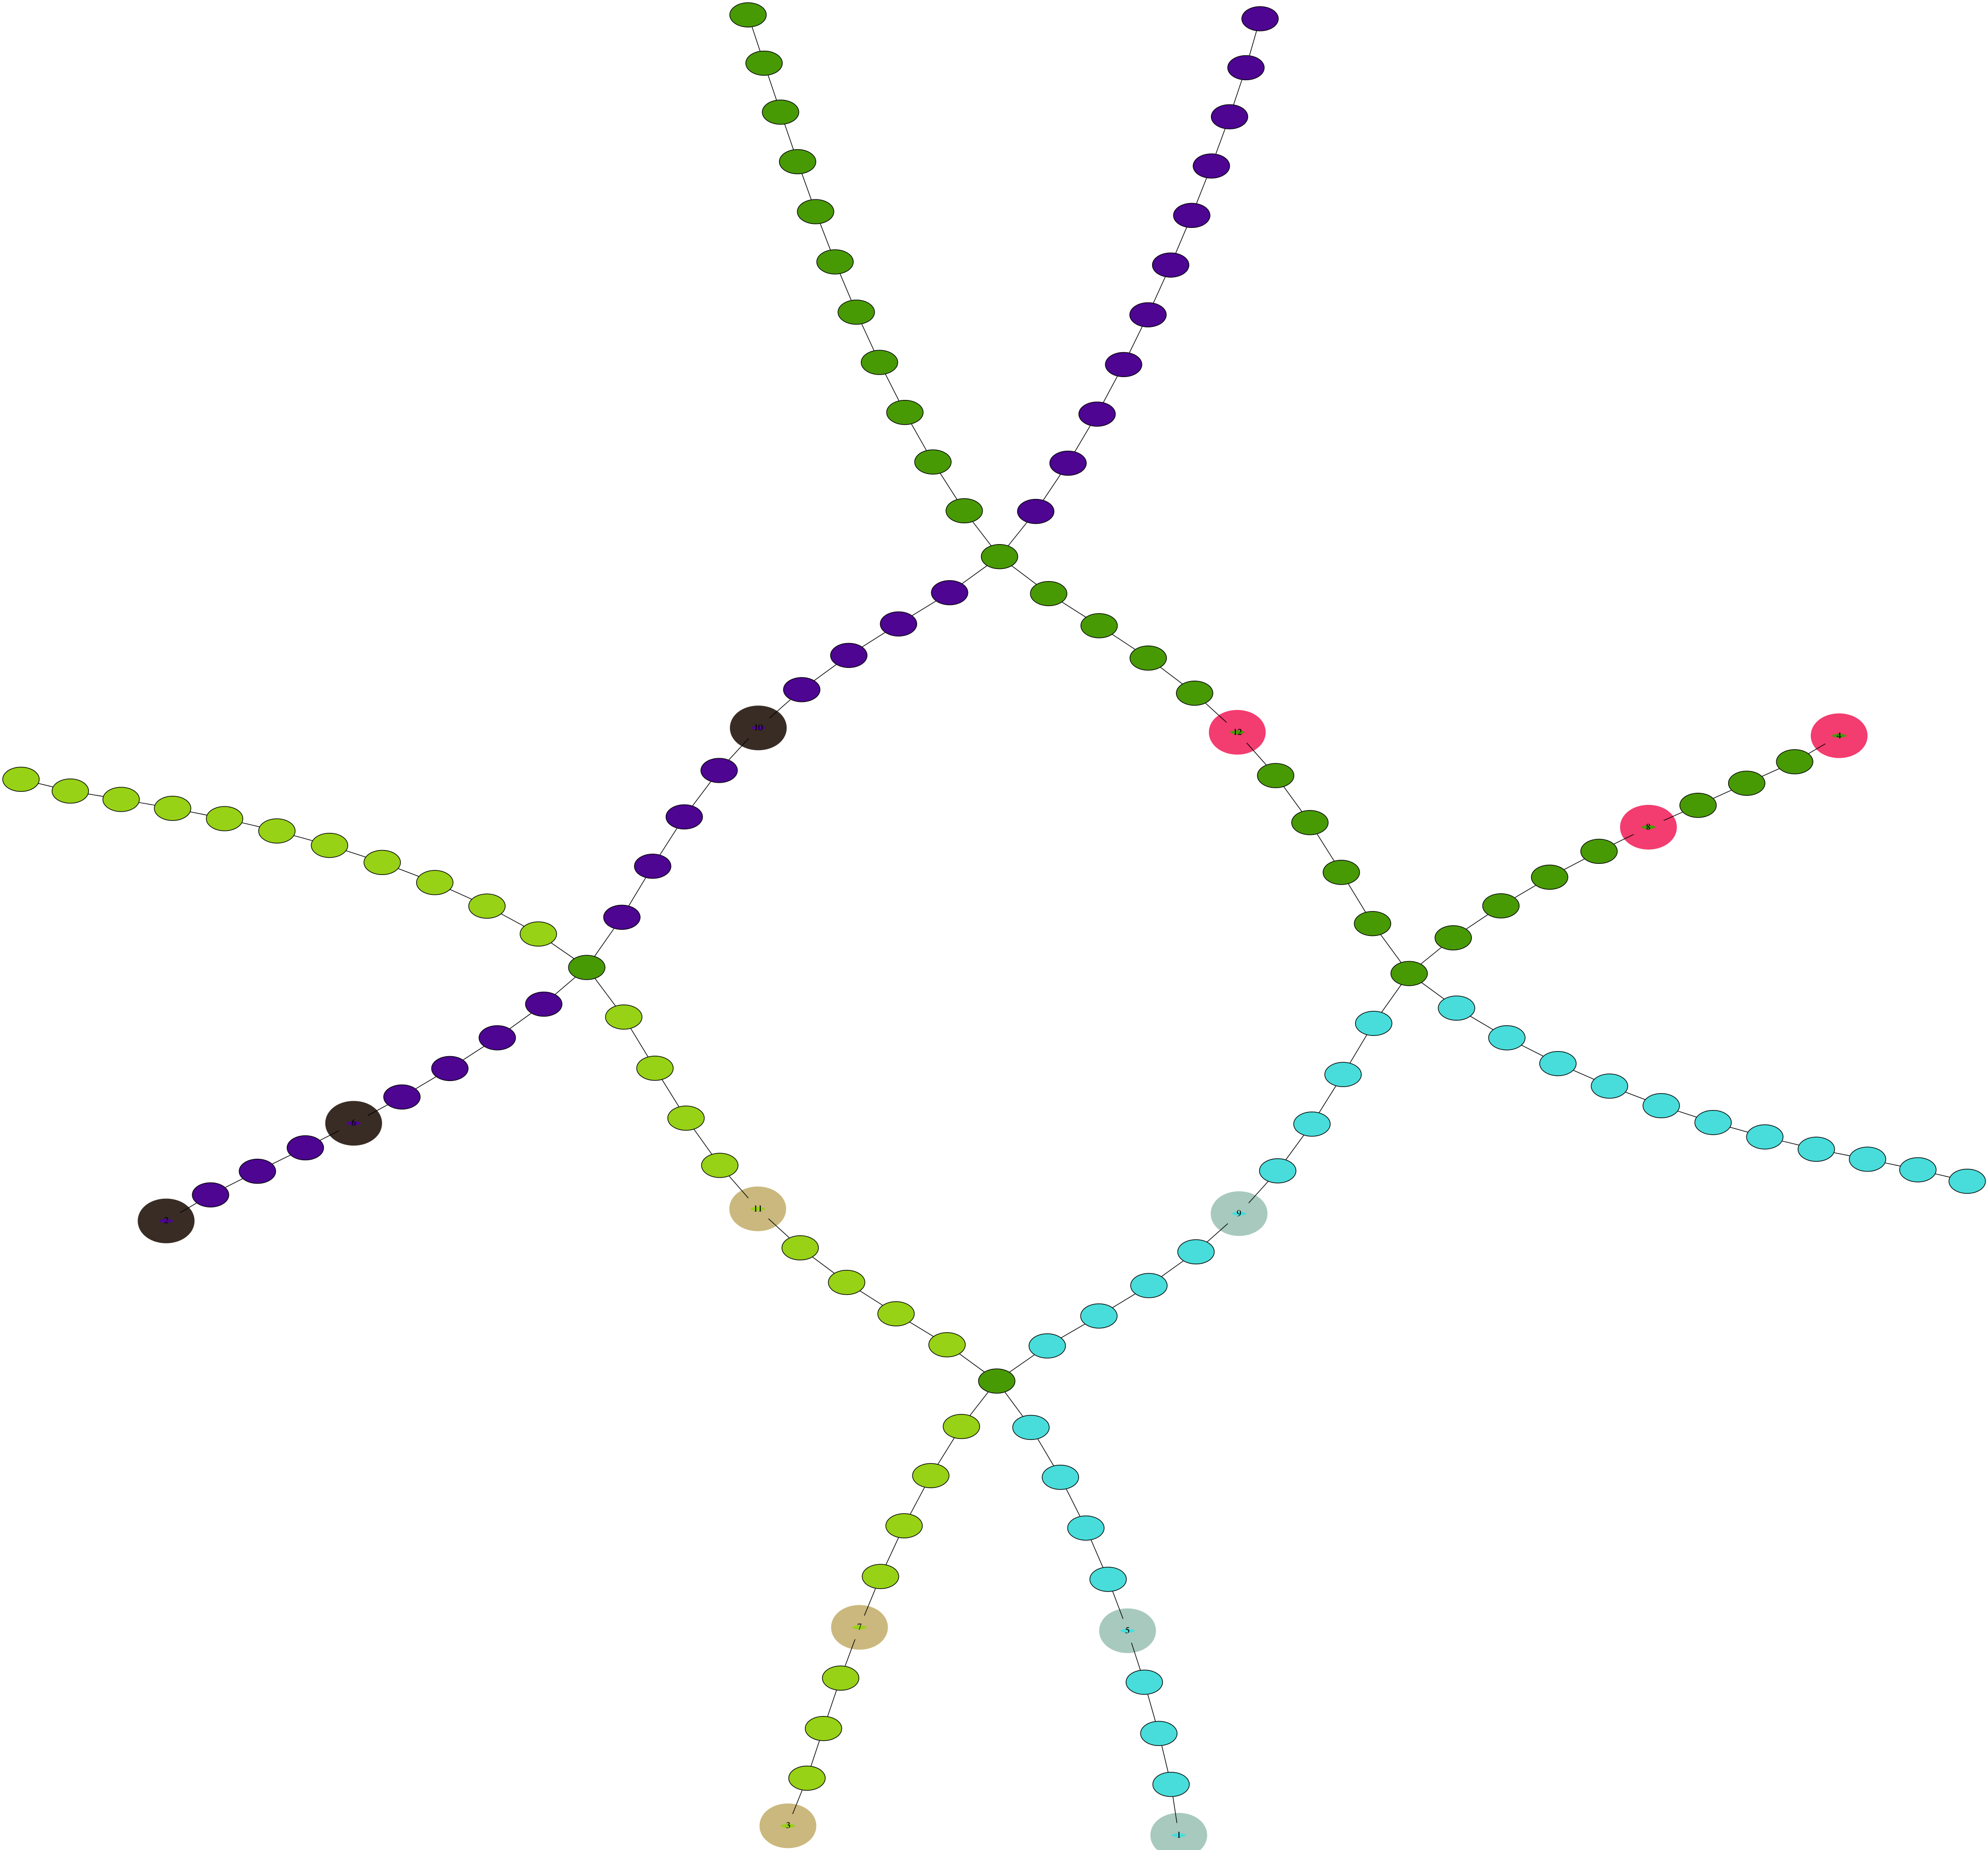
\includegraphics{./model_description/model_example.eps}

\end{document}
